\documentclass{article}
\usepackage{tikz}
\usepackage{pgf-umlcd}
\begin{document}
\section*{Clase abstracta Empleado}
\begin{center}
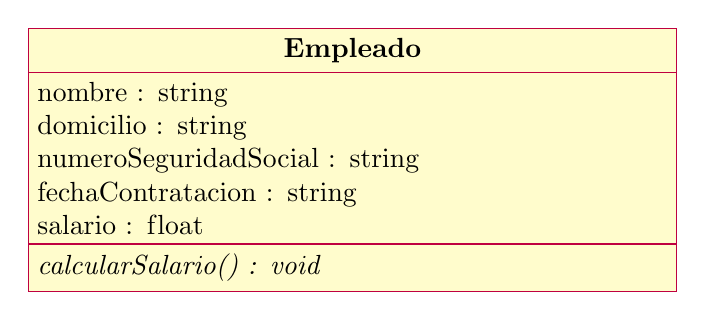
\begin{tikzpicture}
  \begin{class}[text width=8cm]{Empleado}{0,0}
    \attribute{nombre : string}
    \attribute{domicilio : string}
    \attribute{numeroSeguridadSocial : string}
    \attribute{fechaContratacion : string}
    \attribute{salario : f\/loat}
    
    %\operation{name(parameter list) : type of value returned}
    % virtual operations
    %\operation[0]{name(parameters list) : type of value returned}
    \operation[0]{calcularSalario() : void}
  \end{class}
\end{tikzpicture}
\end{center}
\section*{Clase DFecha}
\begin{center}
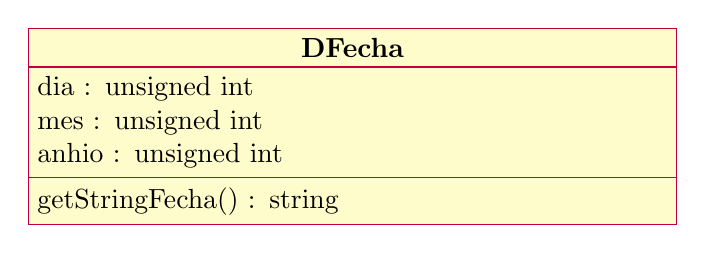
\begin{tikzpicture}
  \begin{class}[text width=8cm]{DFecha}{0,0}
    \attribute{dia : unsigned int}
    \attribute{mes : unsigned int}
    \attribute{anhio : unsigned int}
    %\attribute{fechaContratacion : string}
    %\attribute{salario : f\/loat}
    \operation{getStringFecha() : string}
    %\operation{name(parameter list) : type of value returned}
    % virtual operations
    %\operation[0]{name(parameters list) : type of value returned}
    %\operation[0]{calcularArea() : void}
  \end{class}
\end{tikzpicture}
\end{center}
\section*{Clase abstracta FiguraGeometrica}
\begin{center}
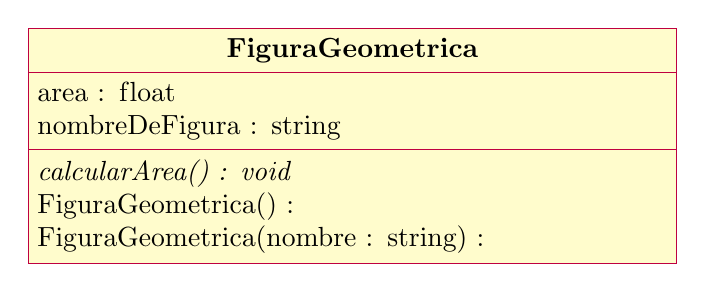
\begin{tikzpicture}
  \begin{class}[text width=8cm]{FiguraGeometrica}{0,0}
    \attribute{area : f\/loat}
    \attribute{nombreDeFigura : string}
    %\attribute{numeroSeguridadSocial : string}
    %\attribute{fechaContratacion : string}
    %\attribute{salario : f\/loat}
    
    \operation[0]{calcularArea() : void}
    \operation{FiguraGeometrica() : }
    % virtual operations
    \operation{FiguraGeometrica(nombre : string) : }
  \end{class}
\end{tikzpicture}
\end{center}
\newpage
\section*{Clase Rectangulo}
\begin{center}
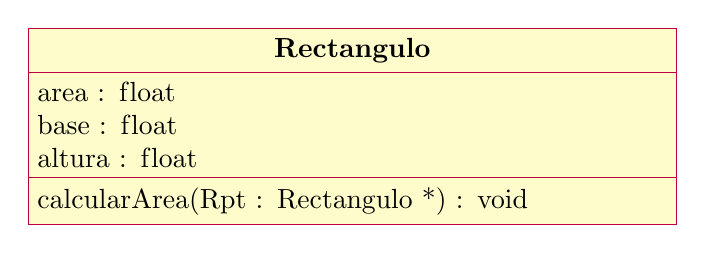
\begin{tikzpicture}
  \begin{class}[text width=8cm]{Rectangulo}{0,0}
    \attribute{area : f\/loat}
    \attribute{base : f\/loat}
    \attribute{altura : f\/loat}
    %\attribute{fechaContratacion : string}
    %\attribute{salario : f\/loat}
    
    %\operation{name(parameter list) : type of value returned}
    % virtual operations
    %\operation[0]{name(parameters list) : type of value returned}
    \operation{calcularArea(Rpt : Rectangulo *) : void}
  \end{class}
\end{tikzpicture}
\end{center}
\begin{verbatim}
/**Rectangulo.h*/
#ifndef RECTANGULO_H
#define RECTANGULO_H
struct Rectangulo {
  float area;
  float base;
  float altura;
};/*end struct Rectangulo*/
void calcularArea(Rectangulo *);    
\end{verbatim}
\end{document}